% mms-euler.tex

\section{Oblique detonation wave}
\index{source terms!user defined!example of use}\index{verification}
\index{chemical reaction!example of use}
\index{gas model!user-defined!example of use}
%
RJG's oblique detonation wave as a code verification exercise for the interaction
of finite-rate chemistry and gas dynamics.
The specified (nonlinear) shape of the ramp should result in a straight shock
when the gas is reacting.
This also shows a use of the user-defined source terms to activate the finite-rate chemical reactions.

\begin{figure}[htbp]
\begin{center}
\mbox{
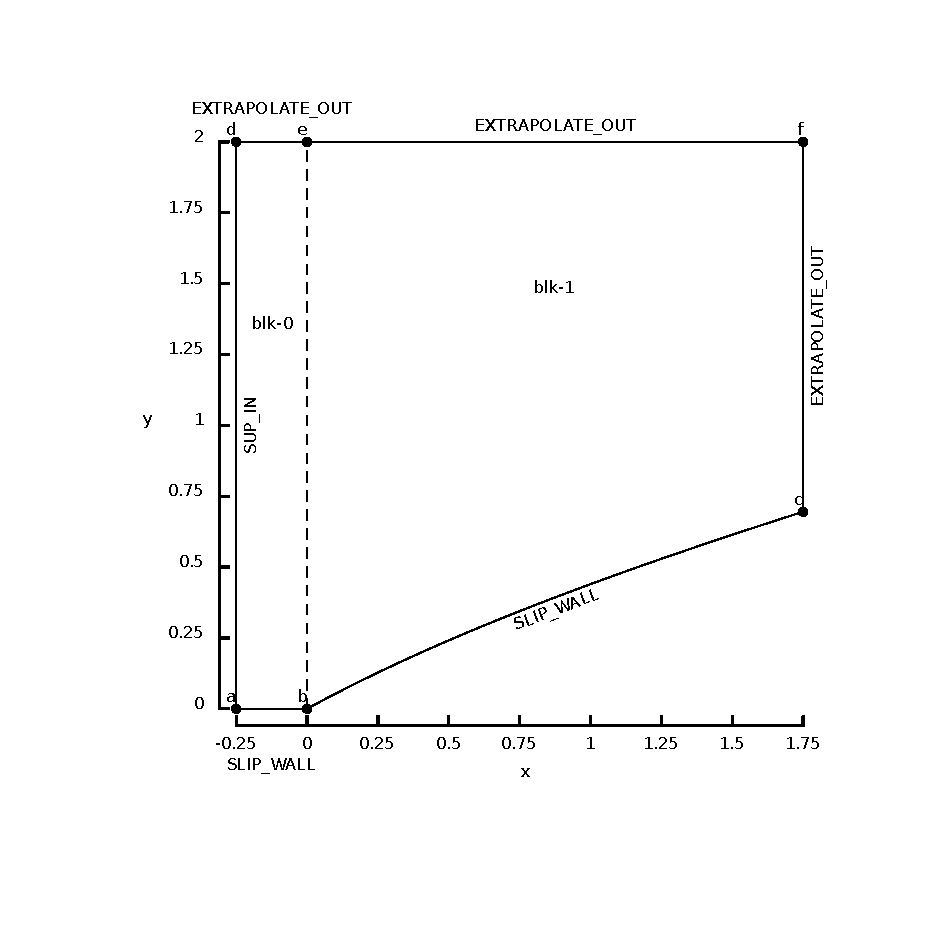
\includegraphics[width=0.6\textwidth,viewport=66 80 396 406]{../2D/odw/odw-layout.pdf}
}
\end{center}
\caption{Layout for the oblique detonation wave simulation.}
\label{odw-layout-fig}
\end{figure}

\begin{figure}[htbp]
\begin{center}
\mbox{
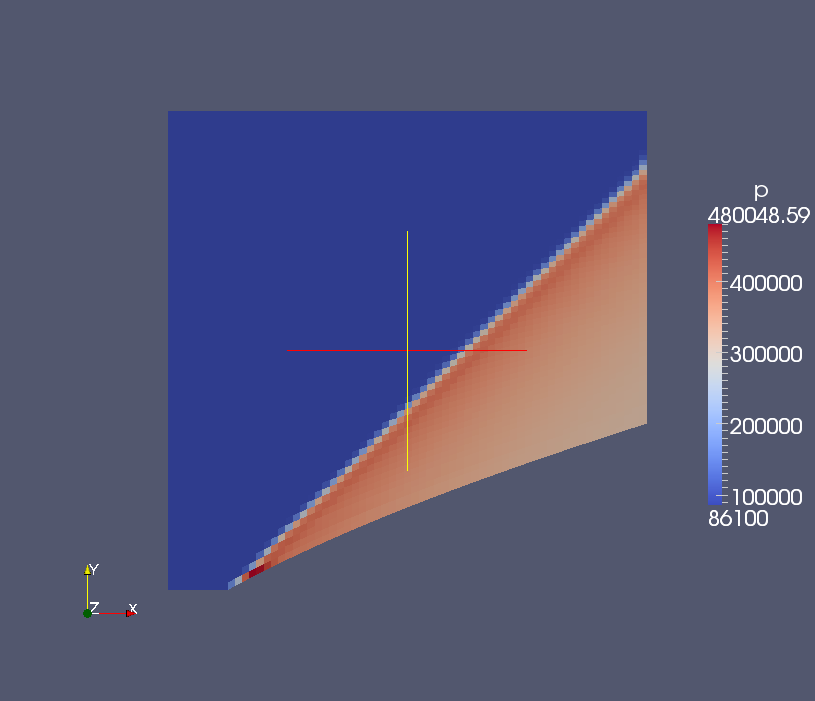
\includegraphics[width=0.5\textwidth]{../2D/odw/odw-t9999-p.png}
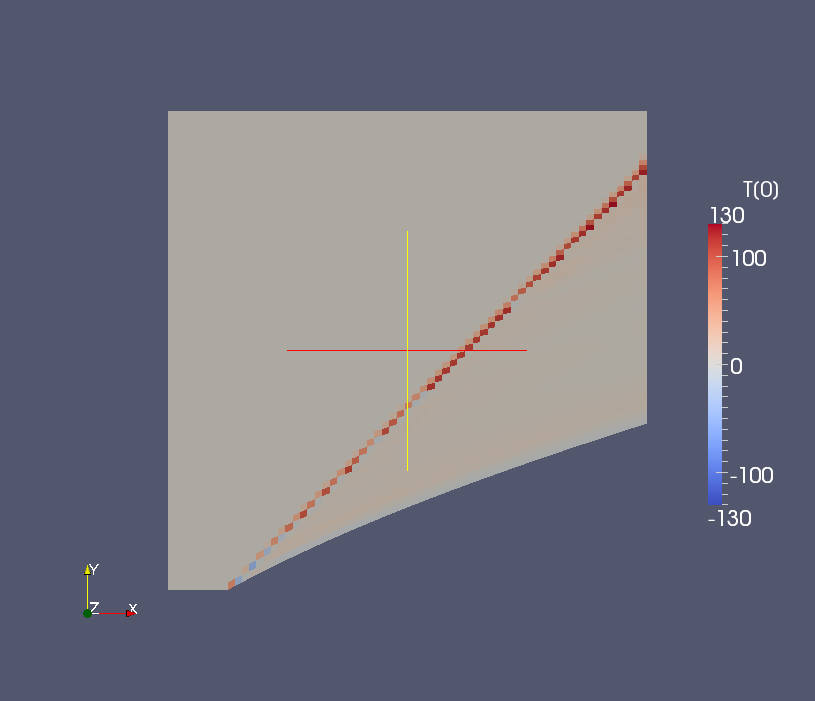
\includegraphics[width=0.5\textwidth]{../2D/odw/odw-t9999-T-diff.png}
}
\end{center}
\caption{Pressure and temperature-difference fields for the steady-state solution.
   The temperature difference is the computed flow temperature minus 
   the analytic solution temperature.}
\label{odw-pressure-T-diff-fig}
\end{figure}


\newpage

\subsection{Input script (.py)}
\topbar
\lstinputlisting[language={}]{../2D/odw/odw.py}
\bottombar

\subsection{gas-model file (binary-gas.lua)}
\topbar
\lstinputlisting[language={}]{../2D/odw/binary-gas.lua}
\bottombar

\subsection{Source term file (.lua)}
%
The source terms are used to activate the chemical reaction.\\
\topbar
\lstinputlisting[language={}]{../2D/odw/udf-source.lua}
\bottombar

\subsection{Shell scripts}
\label{odw-sh-files}
\topbar
\lstinputlisting[language={}]{../2D/odw/prep_simulation.sh}
\bottombar

\noindent
\topbar
\lstinputlisting[language={}]{../2D/odw/run_simulation.sh}
\bottombar

\noindent
The postprocessing script shows features of the post-processor that allow
one to compare one solution with a reference solution described by a Python file.
\index{e3post.py!reference function}

\noindent
\topbar
\lstinputlisting[language={}]{../2D/odw/post_simulation.sh}
\bottombar

\subsection{Python reference function files}
\topbar
\lstinputlisting[language={}]{../2D/odw/odw-ref-function.py}
\bottombar

\noindent
\topbar
\lstinputlisting[language={}]{../2D/odw/oblique_detonation.py}
\bottombar

\subsection{Notes}
\begin{itemize}
\item This simulation required 2\,min, 20\,sec on a single core of 
  a pse-58 (HP workstation) to reach a final time of 10\,ms in 871 steps.
  The cpu time on busemann (Toshiba L500 portable) was 3\,min, 43\,sec.
\end{itemize}
